\subsection{Charakterisierung von Kristallgittern}

Vor der Beschreibung der Oberflächen von Kristallen wenden wir uns dem darunter liegenden 
Gitter zu, das die Basis für die Oberfläche darstellt. Die charakteristischen Größen 
sind auch für die Oberflächen wichtig. Die Untersuchung der Kristallgitter findet vor 
Allem durch Beugungsexperimente statt, da diese die periodische Struktur am besten 
Ausnutzen und so zu höherer Genauigkeit kommen, als direkte Abbildung der Oberflächen. 
Für die gemessene Intensität $I(\mathbf{K})$ gilt für große Abstände $\mathbf{R}$ 
zwischen Strahlungsquelle und streuendem Medium sowie $\mathbf{R'}$ zwischen Streuer 
und Schirm am Ort B:
\begin{equation}
    I(\mathbf{K}) \propto |A_B|^2 \propto |\int \rho(\mathbf{r}) \mathrm{e}^{-i 
    \mathbf{K} \cdot \mathbf{r}} \mathrm{d}\mathbf{r}|^2
\end{equation}
Dabei ist $|A_B|$ die Amplitude der gemessenen Wellen am Schirm, $\rho (\mathbf{r})$ die 
komplexe Streudichte an Position $\mathbf{r}$ (siehe Abb.~\ref{fig:scatter_geometry}) 
und  $\mathbf{K} = \mathbf{k} - \mathbf{k_0}$ der Streuvektor, $\mathbf{k_0}$ der 
k-Vektor der auf das Streumedium auftreffenden Wellen und $\mathbf{k}$ der k-Vektor 
der am Schirm auftreffenden Welle. Für ein periodisches Gitter ist auch die Streudichte
periodisch und lässt sich daher in eine Fourierreihe zerlegen:
\begin{eqnarray}
    \rho(\mathbf{r}) = \sum_{\mathbf{G}} \rho_{\mathbf{G}} \mathrm{e}^{i \mathbf{G} 
        \cdot \mathbf{r}} \\
    \mathbf{r} = n_1 \mathbf{a_1} + n_2 \mathbf{a_2} + n_3 \mathbf{a_3} \\
    \mathbf{G} \cdot \mathbf{r}= 2 \pi m  \\
    n_1, \, n_2, \, n_3, \, m \in \mathbb{N}
\end{eqnarray}
Daraus folgt, dass der Vektor $\mathbf{G}$ als ganzzahlige Linearkombination 
reziproker Gittervektoren $\mathbf{g_i}$ mit der folgenden Bedingung darstellbar ist:
\begin{eqnarray}
    \mathbf{G} = h \mathbf{g_1} + k \mathbf{g_2} + l \mathbf{g_3} \\
    \mathbf{g_i} \cdot \mathbf{a_j} = 2 \pi \delta_{ij}
\end{eqnarray}
Schließlich lassen sich die Basisvektoren des reziproken Gitters berechnen:
\begin{equation}
    \mathbf{g_1} = 2 \pi \frac{\mathbf{a_2 \times a_3} }
        {\mathbf{a_1\cdot (a_2 \times a_3)}}
\end{equation}
Der Zusammenhang mit den experimentell messbaren Daten für $\mathbf{K}$ ist dann wie 
folgt gegeben:
\begin{equation} \label{eqn:G=K}
    I\,(\mathbf{K}) \propto \frac{|A_0|^2}{R'^2} \Big| \sum_{\mathbf{G}} \rho_{\mathbf{G}} 
    \int \mathrm{e}^{i \mathbf{(G - K) \cdot r}} \mathrm{d} \mathbf{r} \Big|^2
\end{equation}
Im Grenzwert unendlich ausgedehnten Volumens wird das Integral zur Deltafunktion, sodass 
für die Intensität gilt:
\begin{equation}
    I\,(\mathbf{K = G}) \propto \frac{|A_0|^2}{R'^2} \,|\rho_{\mathbf{G}} |^2 \, V
\end{equation}

Bei der Bezeichnung von Oberflächen werden die sogenannten Millerschen Indizes benutzt. 
Spannt man mit drei nicht auf einer Geraden liegenden Gitterpunkten, so ist diese durch 
drei ganze Zahlen $m, n, o$ gekennzeichnet. Aus diesen erhält man ein teilerfremdes 
Triplet $(h, k, l)$, indem man die reziproken Werte $h' = 1/m, k' = 1/n, l' = 1/o$ mit 
einer ganzen Zahl $p$ multipliziert. Es lässt sich nun zeigen, dass der reziproke 
Gittervektor $\mathbf{G}$ senkrecht auf dem mit $(h, k, l)$ beschriebenen Gitter steht, 
und für die die in \ref{eqn:G=K} gegebene Bedingung $\mathbf{G = K}$ die Braggsche Reflexionsbedingung 
\begin{equation}
    \gamma = 2 d_{hlk} \sin \Theta
\end{equation}
gilt, wobei 
\begin{equation}
    d_{hkl}=2 \pi / |G_{hkl}|
\end{equation}
der Netzebenenabstand ist und der $\Theta$ der in Abb.~\ref{fig:Bragg_Winkel} definierte
Glanz- oder Braggwinkel ist

\begin{figure}
    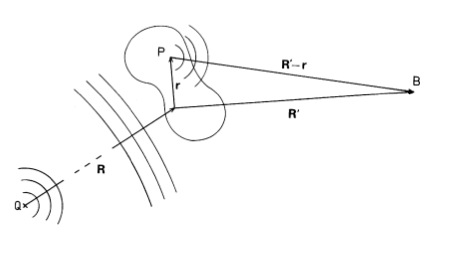
\includegraphics[width=0.8\textwidth]{pics/scatter_geometry}
    \caption{Zur Herleitung der Streukinematik
aus \cite{ibach2009festkorperphysik} }
    \label{fig:scatter_geometry}
\end{figure}

\begin{figure}
    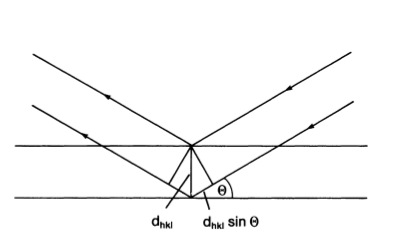
\includegraphics[width=0.8\textwidth]{pics/Bragg_Winkel}
    \caption{Zur Definition des Braggwinkels $\Theta$. Die Netzebenen haben einem Abstand 
von $d_{hlk}$.  
aus \cite{ibach2009festkorperphysik} }
    \label{fig:Bragg_Winkel}
\end{figure}
